% This is samplepaper.tex, a sample chapter demonstrating the
% LLNCS macro package for Springer Computer Science proceedings;
% Version 2.20 of 2017/10/04
%
\documentclass[runningheads]{llncs}
%
\usepackage{graphicx}
% Used for displaying a sample figure. If possible, figure files should
% be included in EPS format.
%
% If you use the hyperref package, please uncomment the following line
% to display URLs in blue roman font according to Springer's eBook style:
\usepackage{hyperref}
% \renewcommand\UrlFont{\color{blue}\rmfamily}


\usepackage[utf8]{inputenc} % Required for inputting international characters
\usepackage[T1]{fontenc} % Output font encoding for international characters

\usepackage[backend=bibtex,natbib=true]{biblatex} % Use the bibtex backend

\addbibresource{bibliography.bib} % The filename of the bibliography

\usepackage[autostyle=true]{csquotes} % Required to generate language-dependent quotes in the bibliography

\usepackage[ruled, linesnumbered,noend]{algorithm2e} % For algorithms

% for function graphs
\usepackage{tikz}
\usepackage{color}
\usetikzlibrary{datavisualization}
\usetikzlibrary{datavisualization.formats.functions}

\usepackage{hhline}
\usepackage{rotating}
\usepackage{multirow}
\usepackage{longtable}
\usepackage{lscape}
\usepackage{adjustbox}
\usepackage{array}
\usepackage{booktabs}

\newcolumntype{R}[2]{%
    >{\adjustbox{angle=#1,lap=\width-(#2)}\bgroup}%
    l%
    <{\egroup}%
}
\newcommand*\rot{\multicolumn{1}{R{90}{1em}}}

\usepackage{dingbat}

\newcommand{\blueline}{\raisebox{2pt}{\tikz{\draw[-,black!40!blue,solid,line width = 0.9pt](0,0) -- (5mm,0);}}}
\newcommand{\yellowline}{\raisebox{2pt}{\tikz{\draw[-,black!40!yellow,solid,line width = 0.9pt](0,0) -- (5mm,0);}}}
\newcommand{\redline}{\raisebox{2pt}{\tikz{\draw[-,black!40!red,solid,line width = 0.9pt](0,0) -- (5mm,0);}}}

\SetKwProg{Fn}{function}{}{}


\begin{document}
%
\title{Learning from Evolving Streams via Self-Training Windowing Ensembles}
%
%\titlerunning{Abbreviated paper title}
% If the paper title is too long for the running head, you can set
% an abbreviated paper title here
%
\author{Sean L. A. Floyd \and
Herna L. Viktor}
%
\authorrunning{SLA Floyd and HL Viktor}
% First names are abbreviated in the running head.
%
\institute{School of Electrical Engineering and Computer Science, University of Ottawa, Ottawa ON, Canada\\
\{sfloy029, hviktor\}@uottawa.ca}
%
\maketitle              % typeset the header of the contribution
%
\begin{abstract}
A major issue with adaptive learning from data streams is late-arriving or missing class labels. Assuming that correctly labelled data will always be available and timely is often unfeasible, and, as such, supervised methods are often not directly applicable to many real-world problems. Such situations thus necessitates the use of semi-supervised or unsupervised learning techniques. Further, the detection of concept drifts in a stream should also not be dependent on labelling information. Based on these observations, we introduce our LESS-TWE framework that employs selective self-training together an unsupervised concept drift detector. Our ensemble-based approach utilised hybrid sliding-windows and use all predictions, rather than only focusing on high predictive confidence.  Our novel windowing technique train each classifier in the ensemble with windows, but delay training in such a way that only one classifier can update its model per prequential loop iteration. This ensures that {\bf Comment: say what do you achieve by doing this}.
Our experimental evaluation indicates that our framework is (roughly 160 times) faster than current state of the art techniques, and achieves comparable predictive accuracy.

\keywords{stream mining \and semi-supervised \and ensembles \and unsupervised drift detection.}
\end{abstract}
%
%
%
\section{Introduction}
%Analytical models have been studied and developed by researchers, with increasing intensity over the last two decades, to intelligently and computationally extract knowledge from data. The quantity and size of data sets have grown exponentially over that time, requiring new algorithms to respect new constraints. Data streams are a latest data format that researchers are developing techniques for, and, are characterised by velocious and continuous flows of data. 
%Researchers have shown a continuing interest in the development of algorithms to extract knowledge from evolving streams  
%Another current topic of interest is the development of ensembles, which are defined as an amalgamation of any number of analytical models.
%These algorithms typically learn in batches by training new classifiers on each incoming chunk, and either use some weighting scheme \cite{chu2004fast,wang2003mining} or replacement strategy that relies on the use of timely and correctly labelled data \cite{chu2004fast, street2001streaming,wang2003mining}. Alternatively, algorithms can learn online by using sliding windows of a variable, or fixed, size to summarise the data and appropriately update their models from them \cite{bifet2009new,nishida2007adaptive}.

Data streams requires algorithms to update their models to adapt to potential changes to the underlying concepts that the stream represent over time. To this end, techniques have been developed to explicitly detect these changes to help models adapt more quickly in order to stay relevant and accurate. Drift detection methods have also mainly relied on the use of labelled data by detecting changes in the accuracy of a classifier over time \cite{bifet2007learning, gama2004learning}. On the other hand drift detectors that are unsupervised, mostly rely on statistical tests \cite{sobolewski2013concept}. A major issue with supervised and semi-supervised learning of data streams is late-arriving or missing class labels. For example, a bank cannot know if a loan will default before several months have passed, if not years. Assuming that correctly labelled data will always be available and timely is unreasonable, and, as such, supervised methods are not usually applicable in the real world. Therefore, real-world problems usually require the use of semi-supervised or unsupervised learning techniques. To the best of our knowledge, no research has been conducted to develop semi-supervised techniques to learn from evolving streams without clustering unlabelled data, which is computationally expensive \cite{krempl2014open}. Furthermore, semi-supervised drift detection algorithms for streams are more applicable to real-world applications, but only one article has been published as of yet \cite{haque2015sand}. {\bf {Comment: say how this is different from your work.}}

%\subsection{Objective\label{section:intro:objective}}
The purpose of this paper is to contribute to narrow the gap in research as it pertains to semi-supervised learning of evolving streams, without clustering unlabelled data.
Our LESS-TWE (Learning from Evolving Streams via Self-Training Windowing Ensembles) framework employs self-training, a novel windowing technique exclusive to ensembles, a soft voting strategy, and an extension of the Fast Hoeffding Drift Detection Method for evolving Streams (FHDDMS) algorithm \cite{pesaranghader2018reservoir}).
Selective self-training learns from labelled data that was originally unlabelled. To do so, it annotates previously unlabelled data with labels for which the classifier has predicted with high confidence \cite{zhu2009selftraining}. Our aim is to study how selective self-training, a semi-supervised learning (SSL) algorithm, performs when removing the selective heuristic, thereby predicting labels for unlabelled data then training on it.  
By introducing the novel windowing technique, we aim to achieve savings relating to the execution time, while maintaining comparable predictive accuracy. Additionally, we observe if delaying the training of some the classifiers in the ensemble affects concept drift detection. {\bf {Comment: concept drift; did you address this in this paper? State explicitly where}}

%\subsection{Organisation}


%As previously stated, this will cover the extension of FHDDMS to reduce its dependency on ground truth, improvements to a simple voting classifier to also further reduce its dependency on ground truth and finally a novel windowing technique that combines sliding and tumbling techniques. 

This paper is organised as follows.  We present our framework in section \ref{section:contributions}.  In section \ref{section:experimental_design}, we will present the experimental design for testing our contributions and present the results and discuss them in section \ref{section:evaluation_discussion}. Finally we identify potential future research in section \ref{section:conclusion}.

\section{LESS-TWE\label{section:contributions}}
%\subsection{Overview of LESS-TWE}

Figure \ref{fig:prequential_loop} illustrates how our contributions fit together and operate in one iteration of an interleaved test-then-train loop.
When predicting labels, data can arrive in chunks or one-by-one. 

As an example, let data arrive one instance at a time. The first step is for the ensemble to predict a label for the new data instance; the classifiers in the ensemble each predict a label and a weighted soft vote scheme selects a winning label for the ensemble. The prediction confidence for that label is used to detect drifts. If a drift is detected, a subset of classifiers in the ensemble are first reset, and subsequently trained on a sliding window of previously seen labelled data (stored in the backup window). If no drifts were detected, then the label predicted replaces the real label value in the novel window, thereby self-training. This window stores the number of instances processed at a time (in this example, one) times $N$, which is the number of classifiers in the ensemble. A single classifier is trained per iteration of the interleaved test-then-train loop, in a cyclical manner, meaning that each classifier in the ensemble is trained only once every $N$ loop iterations. That is, a different classifier from the ensemble is trained at the next loop iteration.

\begin{figure}
  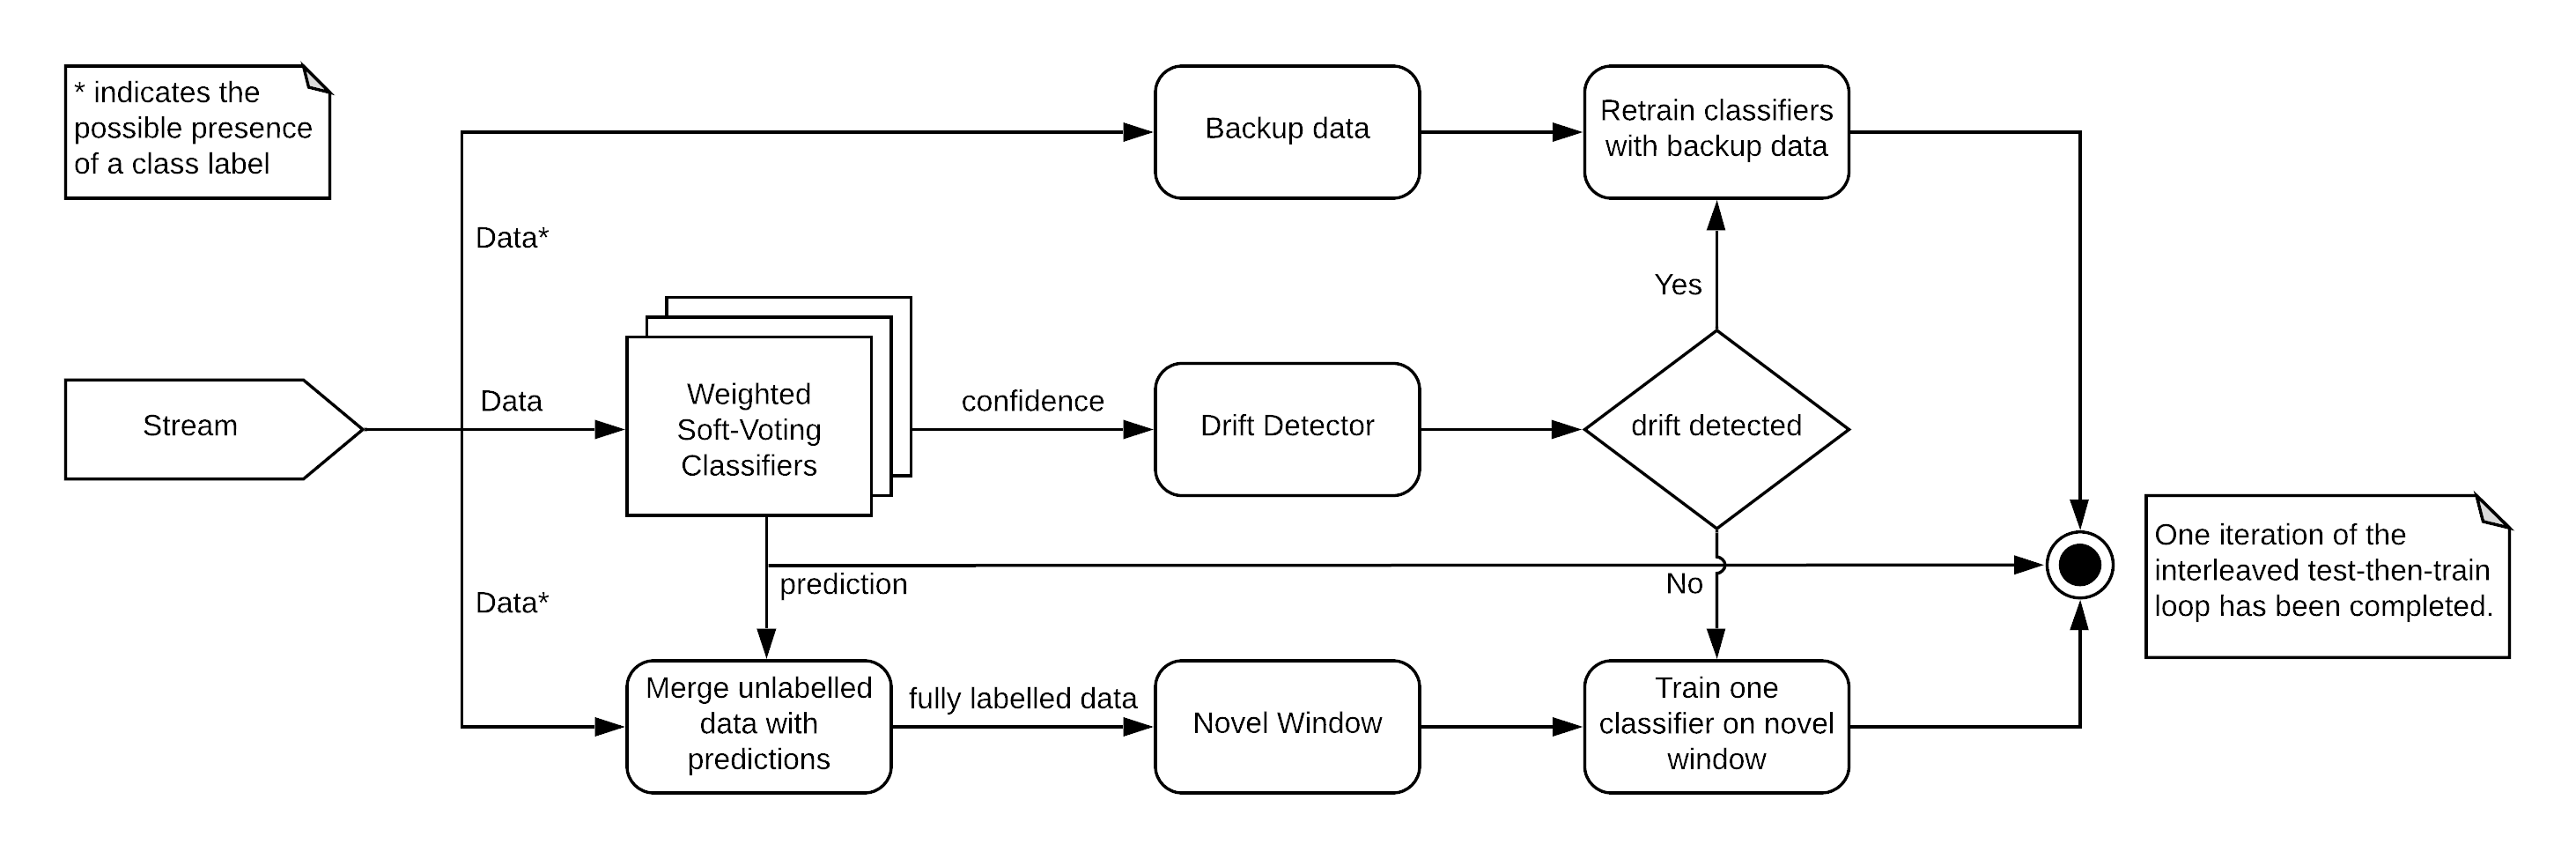
\includegraphics[width=\linewidth]{./images/chapter3/prequential_loop}
\caption{\label{fig:prequential_loop}High-Level Overview of the LESS-TWE methodology}
\end{figure}

\subsection{Drift Detection}
Our drift detection approach extends FHDDM/S as proposed in \cite{pesaranghader2016fast} that relies on the immediate knowledge of labelled data. The drift detection mechanism in FHDDMS relies on storing, in sliding windows, whether or not the classifier correctly predicted the class. A shorter sliding window detects abrupt drifts whereas the longer detects gradual ones. In order to detect drifts without labelled data, we  extend FHDDMS such that its sliding windows now stores a numerical prediction probability value. Therefore, our framework requires classifiers that can output such values. When predicting the class for a data point, each classifier in the ensemble outputs its probability for each class label. For example, a classifier could output the following class probabilities for a non-binary classification task $\{A: 24\%, B: 11\%, C: 65\%\}$.
Our drift detector stores the \textit{average} probability from all classifiers in the ensemble in two sliding windows. The probabilities averaged are those for the winning class of the ensemble soft vote.

\subsection{Hybrid Windowing}

 In \cite{KRAWCZYK2017132}, Krawczyk mentions that one of the many issues in data stream mining is execution time, in the sense that an algorithm must learn faster than tuples can arrive. In our case, we aim to determine if we can delay training of some classifiers in our ensemble, and how it affects execution time and classifying performance.

We propose the following algorithm, implemented in algorithm \ref{alg:sliding_tumbling_windows}.
Let the number of tuples (single tuple or chunk) used in the interleaved test-then-train loop iterations be \textit{number\_of\_tuples}, and let \textit{number\_of\_classifiers} be the number of classifiers in the ensemble. The ensemble will have a window size of \textit{number\_of\_tuples} $\times$ \textit{number\_of\_classifiers}. At every iteration of the interleaved test-then-train loop, we will append the new tuples to the ensemble's window and train a single classifier in the ensemble on that window. For the next \textit{number\_of\_classifiers - 1} iterations, we will train the remaining \textit{number\_of\_classifiers - 1} classifiers in the ensemble. We do this so that from the point of view of the ensemble, we are training using sliding windows. However, from the point of each classifier in the ensemble, we are training them using tumbling windows.

While not used for the same purpose, the same sliding batches were used to improve CDC-Stream in \citep{d2017context}. Figure \ref{fig:sliding_tumbling_windows}, shows how the algorithm works for three (3) classifiers in the ensemble with a batch size of one (1) and a window size of three (3). Each classifier will only learn from the same coloured batch; meaning that at time \textit{t}, only a single classifier has enough tuples to learn from, but the others will learn at time \textit{t+1} and finally at time \textit{t+2}. Each classifier will be learning from what essentially is a tumbling window, from their point of view, just not all from the same one, or at the same time. 

%To clarify the example, (using figure \ref{fig:sliding_tumbling_windows}) at time $t_1$, our ensemble will receive only one instance, add it to the sliding window and train classifier $c_1$ on the window. At time $t_2$, another instance will be added to the window and the ensemble will train classifier $c_2$ on the new window containing two tuples. At time $t_3$, the ensemble will train classifier $c_3$ on the first purple chunk (the window now has its maximum of 3 instances). At time $t_4$, $c_2$ will learn from the first blue chunk. And at time $t_5$, $c_3$ will learn from the first green chunk. This process loops indefinitely. 

\begin{algorithm}
\KwResult{at least one classifier in the ensemble was trained}
\tcp{voting\_ensemble stores a classifier list, its count, and, the index of the current classifier to train}
\Fn{ensemble.train(X, y)}{    
        classifier\_to\_train = classifier\_list[index]\;
        index = (index + 1) modulo (number\_of\_classifiers)\;
        classifier\_to\_train.partial\_train(X, y)\;
}
\caption{Sliding-Tumbling Windows for Training Ensembles\label{alg:sliding_tumbling_windows} }
\end{algorithm}


\begin{figure}
\begin{center}
 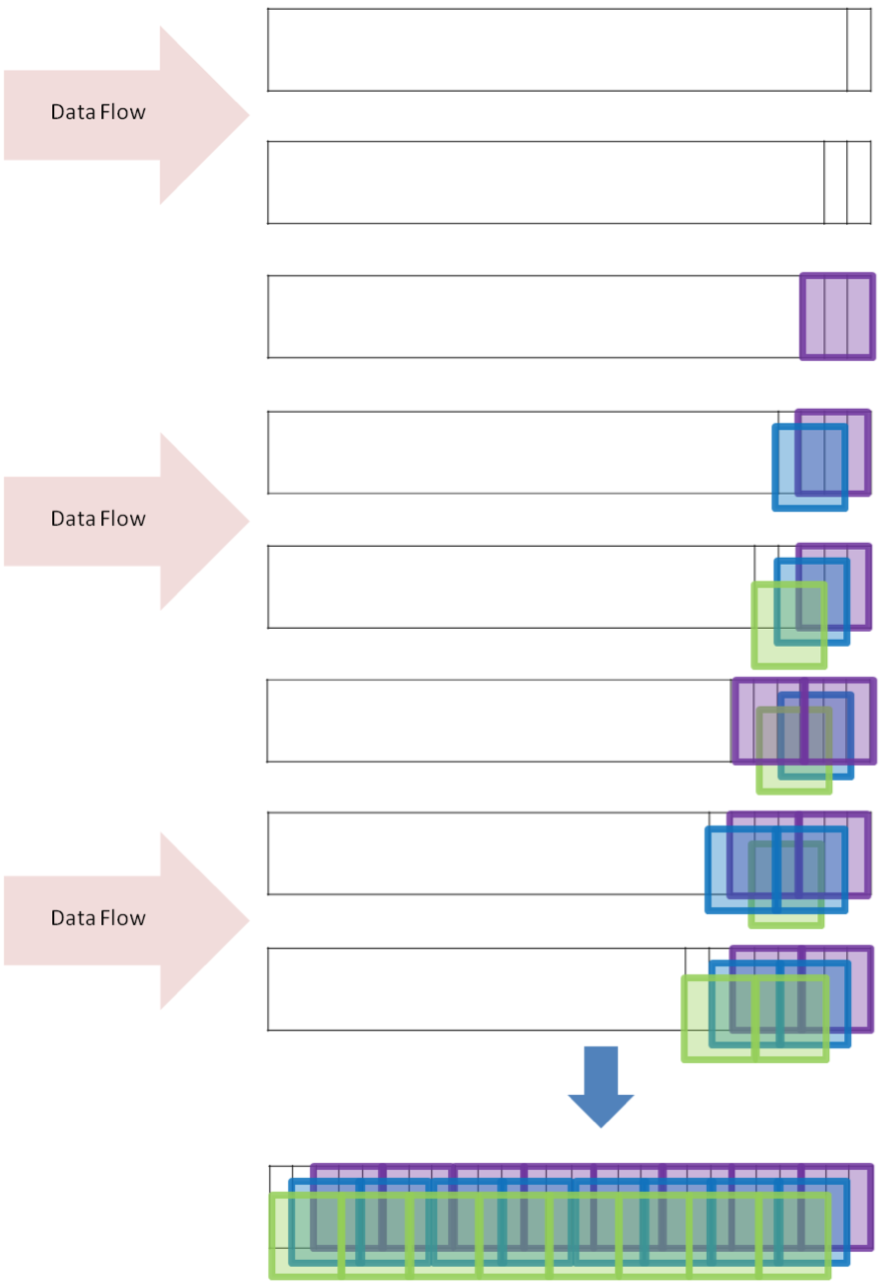
\includegraphics[width=6.5cm]{./images/chapter3/sliding_tumbling_windows}
 \caption{Sliding Tumbling windows \citep{d2017context}.}
 \label{fig:sliding_tumbling_windows}
 \end{center}
\end{figure}

\subsection{Self-Training}

{\bf{Need to be updated, with references: explain what you do, this is more "background"}}

{\bf{We extend offline self-training to reduce our dependency on labelled data for training in an online streaming setting. To this end, we use the classifier's prediction, as opposed to correctly labelled instances, when training.
However, self-training, at least in an offline setting, can reinforce classification errors; it is, therefore, logical for us to conclude that we will encounter the same risks in porting this idea to a streaming setting {\bf{add reference}}. Given this restriction of limiting reinforcing misclassification errors, our goal is to determine at what ratio of predictions to ground-truth our voting ensemble's accuracy would decline and by how much.
Our algorithm consists of duplicating the class label array and replacing at random a given fraction of true labels with predictions from the ensemble, if a drift was not detected. Refer to algorithm \ref{alg:self-training} for the pseudocode.}}

\begin{algorithm}
\While{stream.has\_more\_instances()}{
    X, y = stream.get\_next\_tuples(number\_of\_instances\_to\_fetch)\;
    predictions, probabilities = voting\_ensemble.predict(X)\;
    drift\_detected = voting\_ensemble.detect\_drift(predictions, probabilities)\;
    \If{$percentage \neq 100$ \textbf{and} drift not detected}{
        y = swap\_ground\_truth\_with\_predictions(y, predictions, percentage)\;
    }
 voting\_ensemble.train(X, y)\;
}

\tcp{This algorithm only shows the steps required to modify the ground truth array}
\Fn{swap\_ground\_truth\_with\_predictions(y, predictions, percentage)}{
    \For{$index=0\ \textbf{;}\ index < length(y)\ \textbf{;}\ index += 1$}{
        \If{random\_number\_between(0, 100) > percentage}{
            y[index] = predictions[index]\;
        }
    }
    \Return{y}\;
}
\caption{\label{alg:self-training}Online self-training}
\end{algorithm}

\section{Experimental Evaluation\label{section:experimental_design}}
%In this section, we describe our experimental design.

All experiments were conducted on a \href{https://everymac.com/systems/apple/macbook_pro/specs/macbook-pro-core-i7-2.2-15-iris-only-mid-2015-retina-display-specs.html}{MacBook Pro base model \textit{11,4}}, running macOS 10.14.4. The framework's implementation and the code for the experiments are available at GitHub\footnote{\url{https://github.com/SeanLF/scikit-multiflow}}.
Our Voting Ensemble is composed of three classifiers: Stochastic Gradient Descent, Multinomial Naive Bayes, and Gaussian Naive Bayes. Finally, we also used a no-change classifier as well as a majority-class classifier as our baselines.

The estimation technique we use is prequential evaluation, which consists of infinitely executing a loop where a classifier first predicts labels for new data (without its label), then adapts its model for said data, with the correct label.
The performance measures that we use are the execution time, measured in seconds, as well as the $\kappa$-temporal statistic to evaluate a classifier's predictive performance, also called $\kappa^+$ or $\kappa_t$. This $\kappa$ statistic compares our classifier to a no-change classifier and takes into account temporal dependence in the data.
%\cite{vzliobaite2015evaluation}.

We compare our ensemble to the state of the art leveraging bagging (LB) algorithm, using parameter combinations selected by inspection after having been ranked with an averaging equation \ref{eq:rank_both}. We also compare these results with no-change and majority-class classifiers (trained with 100\% labelled examples and sliding windows). The leveraging bagging classifier is implemented with a built-in ADWIN drift detector and uses ten Hoeffding Tree estimators. We employ the Friedman test in conjunction with the post-hoc Nemenyi test to determine the statistical significance of our results.

%\subsection{Data Sets}
The data sets used for our analysis are SEA \cite{street2001streaming}, CIRCLES, SINE1 and MIXED \cite{10.1007/3-540-59286-5_74}, which all contain noise, and either abrupt or gradual concept drifts. We have generated data for SEA, while the data generated for the last three data sets was obtained from \cite{pesaranghader2016fast}. Finally, each experiment is run on five different examples each sourced from three synthetic data sets (5 examples of $SINE1$, another 5 of $CIRCLES$, etc.) and three streams generated by the SEA generator with levels of noise in increments of ten percent (from 0\% to 20\%), for a grand total of eighteen (18) streams of one hundred thousand (100000) instances.

\subsubsection{$CIRCLES$}
 is composed of two relevant numerical attributes: $x$ and $y$, which are uniformly distributed in [0, 1]. There are four different concepts in this data set, each representing whether or not a point is within a circle given $x$, and $y>$ coordinates for its centre and its radius $r_c$. This data set contains gradual concept drifts that occur at every twenty-five thousand (25 000) instances. The four pairs of $<(x,y), r_c>$ defining each concept are given in table \ref{table:circle_concepts}.

%\begin{table}[]
%\centering
%\caption{\label{table:circle_concepts}$CIRCLES$ data set concepts}
%\begin{tabular}{|c|c|c|c|c|}
%\hline
%center & (0.2, 0.5) & (0.4, 0.5) & (0.6, 0.5) & (0.8, 0.5) \\ \hline
%radius & 0.15       & 0.2        & 0.25       & 0.3        \\ \hline
%\end{tabular}
%\end{table}

\subsubsection{$SINE1$}
contains abrupt concept drifts. It has only two relevant numerical attributes, for which the values are uniformly distributed in [0, 1]. Before the concept drift, all instances for values below the curve $y = sin(x)$ are classified as \textbf{positive}. Then, after the concept drift, the rule is reversed; therefore the values below the curve become \textbf{negative}. The drifts were generated at every twenty thousand (20 000) instances.

\subsubsection{$MIXED$}
contains abrupt concept drifts and uses four relevant attributes, two of which are boolean, let them be $v$ and $w$; and the other two attributes are numerical, in [0, 1]. Instances belong to the positive class if two of three conditions are met: $v$ is true, $w$ is true, $y < 0.5 + 0.3 \times sin(3\pi x)$. For each concept drift, the conditions are reversed, meaning that if the conditions are met, it will be a positive instance, then after the drift, it will be a negative instance. The abrupt concept drifts occur at every twenty thousand (20 000) instances.

\subsubsection{Streaming Ensemble Algorithm (SEA)}
generates streams with abrupt concept drift, composed of three numerical attributes of values in [0, 10], where only the first two attributes are relevant. For each instance, the class is determined by checking if the sum of the two relevant attributes passes a threshold value. Let $f_1$ and $f_2$ be the two numerical relevant attributes, and $\theta$ the threshold. An instance belongs to class \textit{one} if $f_1 + f_2 \leq \theta$. As in \cite{street2001streaming}, our stream has four concepts, with the threshold values for each being 8, 9, 7 and 9.5. We generate streams of one hundred thousand instances, from zero to twenty percent noise, in ten percent increments ($\{0; 10; 20\%\}$). Drifts, therefore, occur at every twenty-five thousand instances.

%\subsection{Experimental Results\label{section:evaluation_discussion}}

%Recall that in the previous section, in order to evaluate our contributions, we measure how our algorithm performs over four different data sets, using the $\kappa_t$ metric, as well as the execution time, while also considering the percentage of labelled data used to train our ensemble.

%Next, we present our experimental results.

\subsection{Effects of training with less labelled data}
\begin{figure}
  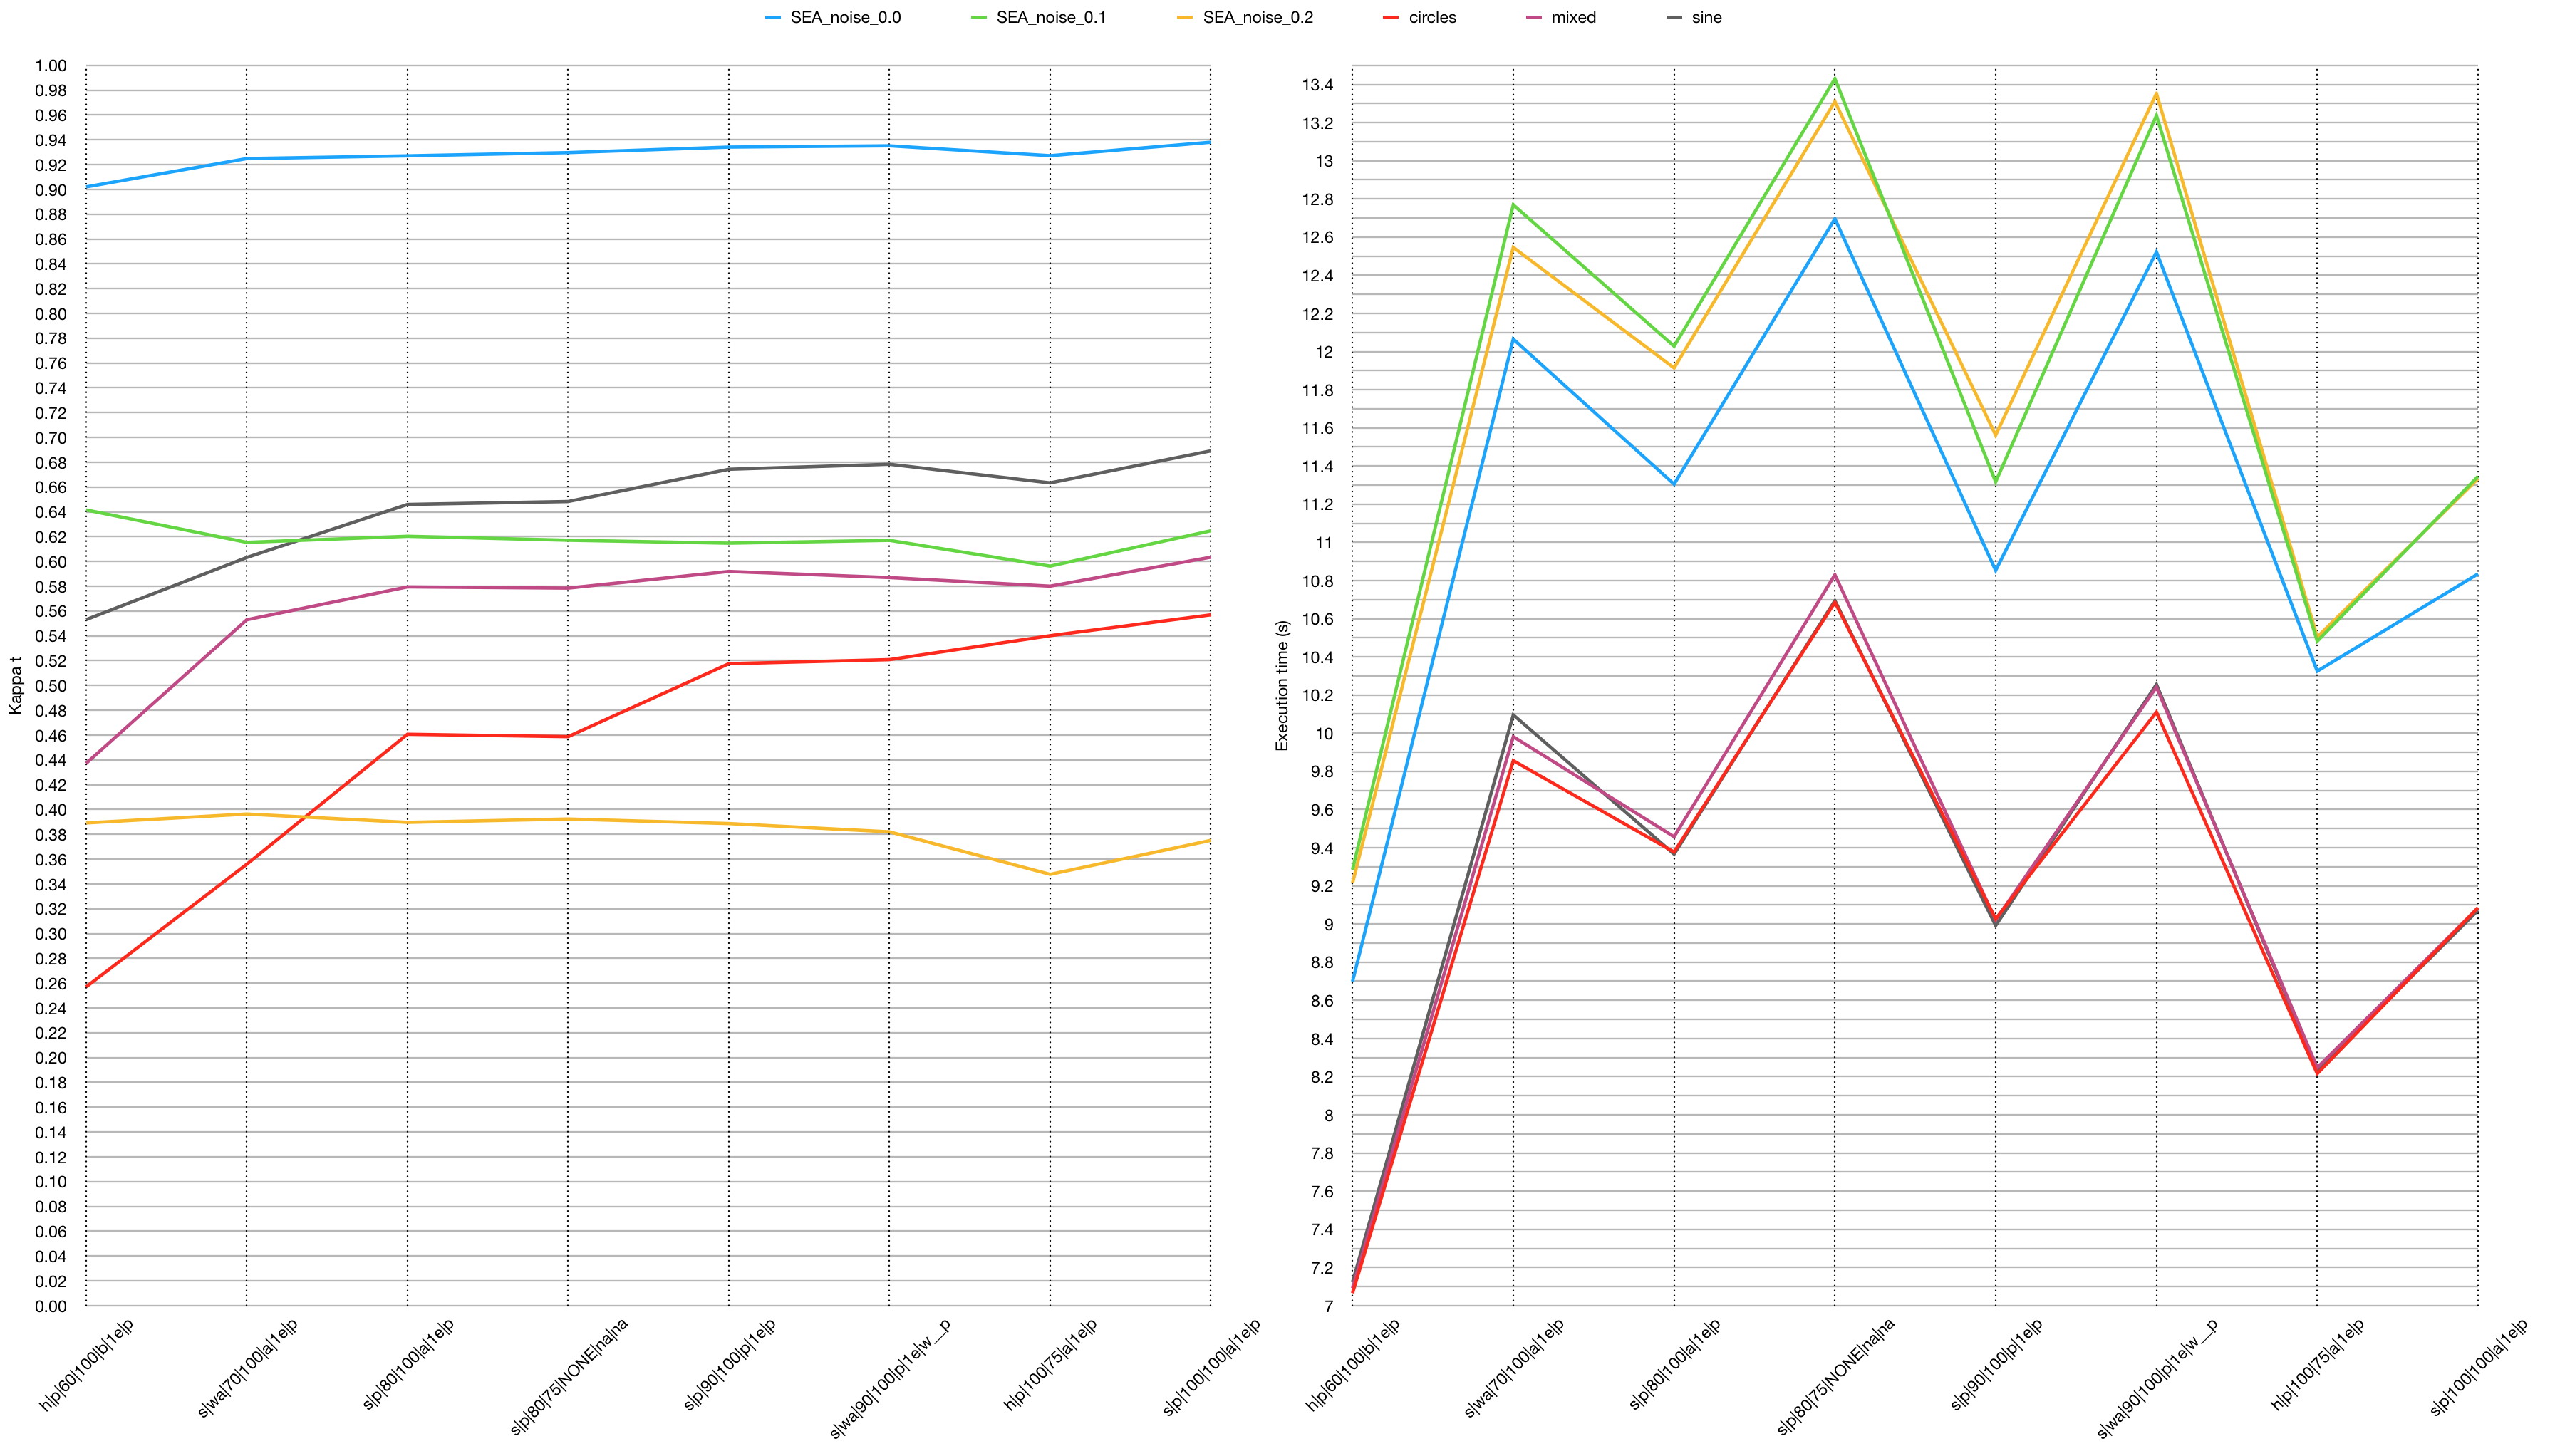
\includegraphics[width=\linewidth]{./images/chapter5/ground_truth_both}
\caption{\label{fig:ground_truth_drop}$\kappa_t$ and execution times for parameter combinations using varying amounts of ground truth}
\end{figure}

Recall that we aim to determine the percentage of labelled data used at which our voting ensemble's $\kappa_t$ metric declines. Figure \ref{fig:ground_truth_drop} shows the predictive performance and execution times for parameter combinations with varying amounts of ground truth (ten percent increments starting at 60\%). The parameter combinations were selected by inspection after having been ranked with an averaging equation (\ref{eq:rank_both}) that assigns more weight to the rank for the $\kappa_t$ metric than that of the execution time. The ranking algorithm from the Nemenyi test was extracted to rank the possible parameter combinations.
\begin{equation}
\label{eq:rank_both}
\frac{3\times rank_{\kappa_t}+rank_{execution\ time}}{4}
\end{equation}

Table \ref{table:ground_truth_Acc_kappa} lists the global predictive accuracy and the $\kappa_t$ values for each data set for some of the parameter values used in figure \ref{fig:ground_truth_drop}. This table indicates that the global predictive accuracy of our ensemble is not significantly reduced by training with less ground truth. However, the predictive performance of the ensemble, as measured by $\kappa_t$, differs between 20\% and 54\% when examining $\kappa_t$ when using 60\% and 100\% of ground truth. The $\kappa_t$ results indicate that as the ensemble trains with less labelled data, it performs more similarly to a baseline no-change classifier.

\begin{table}
  \centering
  \caption{Accuracy (\%) and $\kappa_t$ when training with varying percentages of labelled data for the parameter combinations in figure \ref{fig:ground_truth_drop}.
  \label{table:ground_truth_Acc_kappa}}
  \begin{tabular}{|c||c|c|c|c|c|c|c|c|c|c|c|c|}
  \hline
   & \multicolumn{2}{c|}{\textbf{CIRCLES}} & \multicolumn{2}{c|}{\textbf{MIXED}} & \multicolumn{2}{c|}{\textbf{SINE1}} & \multicolumn{2}{c|}{\textbf{SEA 0\%}} & \multicolumn{2}{c|}{\textbf{SEA 10\%}} & \multicolumn{2}{c|}{\textbf{SEA 20\%}} \\ \cline{2-13} 
\multirow{-2}{*}{\textbf{GT}} & \multicolumn{1}{c|}{\textbf{Acc}} & \multicolumn{1}{c|}{\textbf{$\kappa_t$}} & \multicolumn{1}{c|}{\textbf{Acc}} & \multicolumn{1}{c|}{\textbf{$\kappa_t$}} & \multicolumn{1}{c|}{\textbf{Acc}} & \multicolumn{1}{c|}{\textbf{$\kappa_t$}} & \multicolumn{1}{c|}{\textbf{Acc}} & \multicolumn{1}{c|}{\textbf{$\kappa_t$}} & \multicolumn{1}{c|}{\textbf{Acc}} & \multicolumn{1}{c|}{\textbf{$\kappa_t$}} & \multicolumn{1}{c|}{\textbf{Acc}} & \multicolumn{1}{c|}{\textbf{$\kappa_t$}} \\ \hhline{=============}
  \textbf{100} & {\color[HTML]{656565} 78} & 0.56 & {\color[HTML]{656565} 80} & 0.60 & {\color[HTML]{656565} 84} & 0.69 & {\color[HTML]{656565} 97} & 0.94 & {\color[HTML]{656565} 82} & 0.62 & {\color[HTML]{656565} 70} & 0.38 \\ \hline
  \textbf{90} & {\color[HTML]{656565} 76} & 0.52 & {\color[HTML]{656565} 79} & 0.59 & {\color[HTML]{656565} 84} & 0.68 & {\color[HTML]{656565} 97} & 0.94 & {\color[HTML]{656565} 82} & 0.62 & {\color[HTML]{656565} 70} & 0.38 \\ \hline
  \textbf{80} & {\color[HTML]{656565} 73} & 0.46 & {\color[HTML]{656565} 79} & 0.58 & {\color[HTML]{656565} 82} & 0.65 & {\color[HTML]{656565} 96} & 0.93 & {\color[HTML]{656565} 82} & 0.62 & {\color[HTML]{656565} 70} & 0.39 \\ \hline
  \textbf{70} & {\color[HTML]{656565} 68} & 0.36 & {\color[HTML]{656565} 77} & 0.55 & {\color[HTML]{656565} 80} & 0.60 & {\color[HTML]{656565} 96} & 0.92 & {\color[HTML]{656565} 82} & 0.62 & {\color[HTML]{656565} 71} & 0.40 \\ \hline
  \textbf{60} & {\color[HTML]{656565} 63} & 0.26 & {\color[HTML]{656565} 72} & 0.44 & {\color[HTML]{656565} 77} & 0.55 & {\color[HTML]{656565} 95} & 0.90 & {\color[HTML]{656565} 83} & 0.64 & {\color[HTML]{656565} 70} & 0.39 \\ \hline
  \end{tabular}
  \end{table}

%One finding that we find particularly odd is that as the use of ground truth diminishes, the predictive accuracy increases for the SEA generated data sets with noise. We are led to believe that for increasing levels of noise in a data set, reducing the ground truth used (to an extent) to train a model increases its predictive performance. Further research, outside the scope of this paper, is needed to ascertain the veracity of this finding.

From figure \ref{fig:ground_truth_drop} and table \ref{table:ground_truth_Acc_kappa}, we find that our ensemble does not suffer a drastic reduction in its global predictive accuracy when training with only 60\% ground truth (in other words, training with 40\% less labelled data). However, the $\kappa_t$ statistic indicates that training our ensemble using non-selective self-training on a data set containing less than 70\% labelled data results in a predictive performance that is not drastically better than a no-change classifier (for the most part, as results for SEA and the other data sets highly differ). Additionally, one notes that the CIRCLES data set is harder to model with access to less labelled data, which is perfectly logical given what the class label represents. Indeed, very specific data instances are required to model the class well, given that it represents whether or not a data instance resides within the radius of a predefined circle. It is clear that the reduction in $\kappa_t$ is dependant on both the data set being modelled as well as how much of that data set is labelled. Overall, we find that training our ensemble with a data set that is 80\% or 90\% labelled leads to a good predictive accuracy (as measured by $\kappa_t$).

\subsection{Comparing to the State of the Art}

%As previously mentioned, the algorithm which we will be comparing our voting ensemble to will be mainly Leveraging Bagging. As we stated in section \ref{section:experimental_design}, the Leveraging Bagging ensembles will be comprised of 10 Hoeffding Tree estimators, each with its own ADWIN drift detector. We will also be using a regular Hoeffding Tree using its default parameters without any drift detector. Finally, we will also include a no-change and a majority class classifier in our comparison.

%\subsubsection{Choosing a window size for State of the Art algorithms}

\begin{figure}
  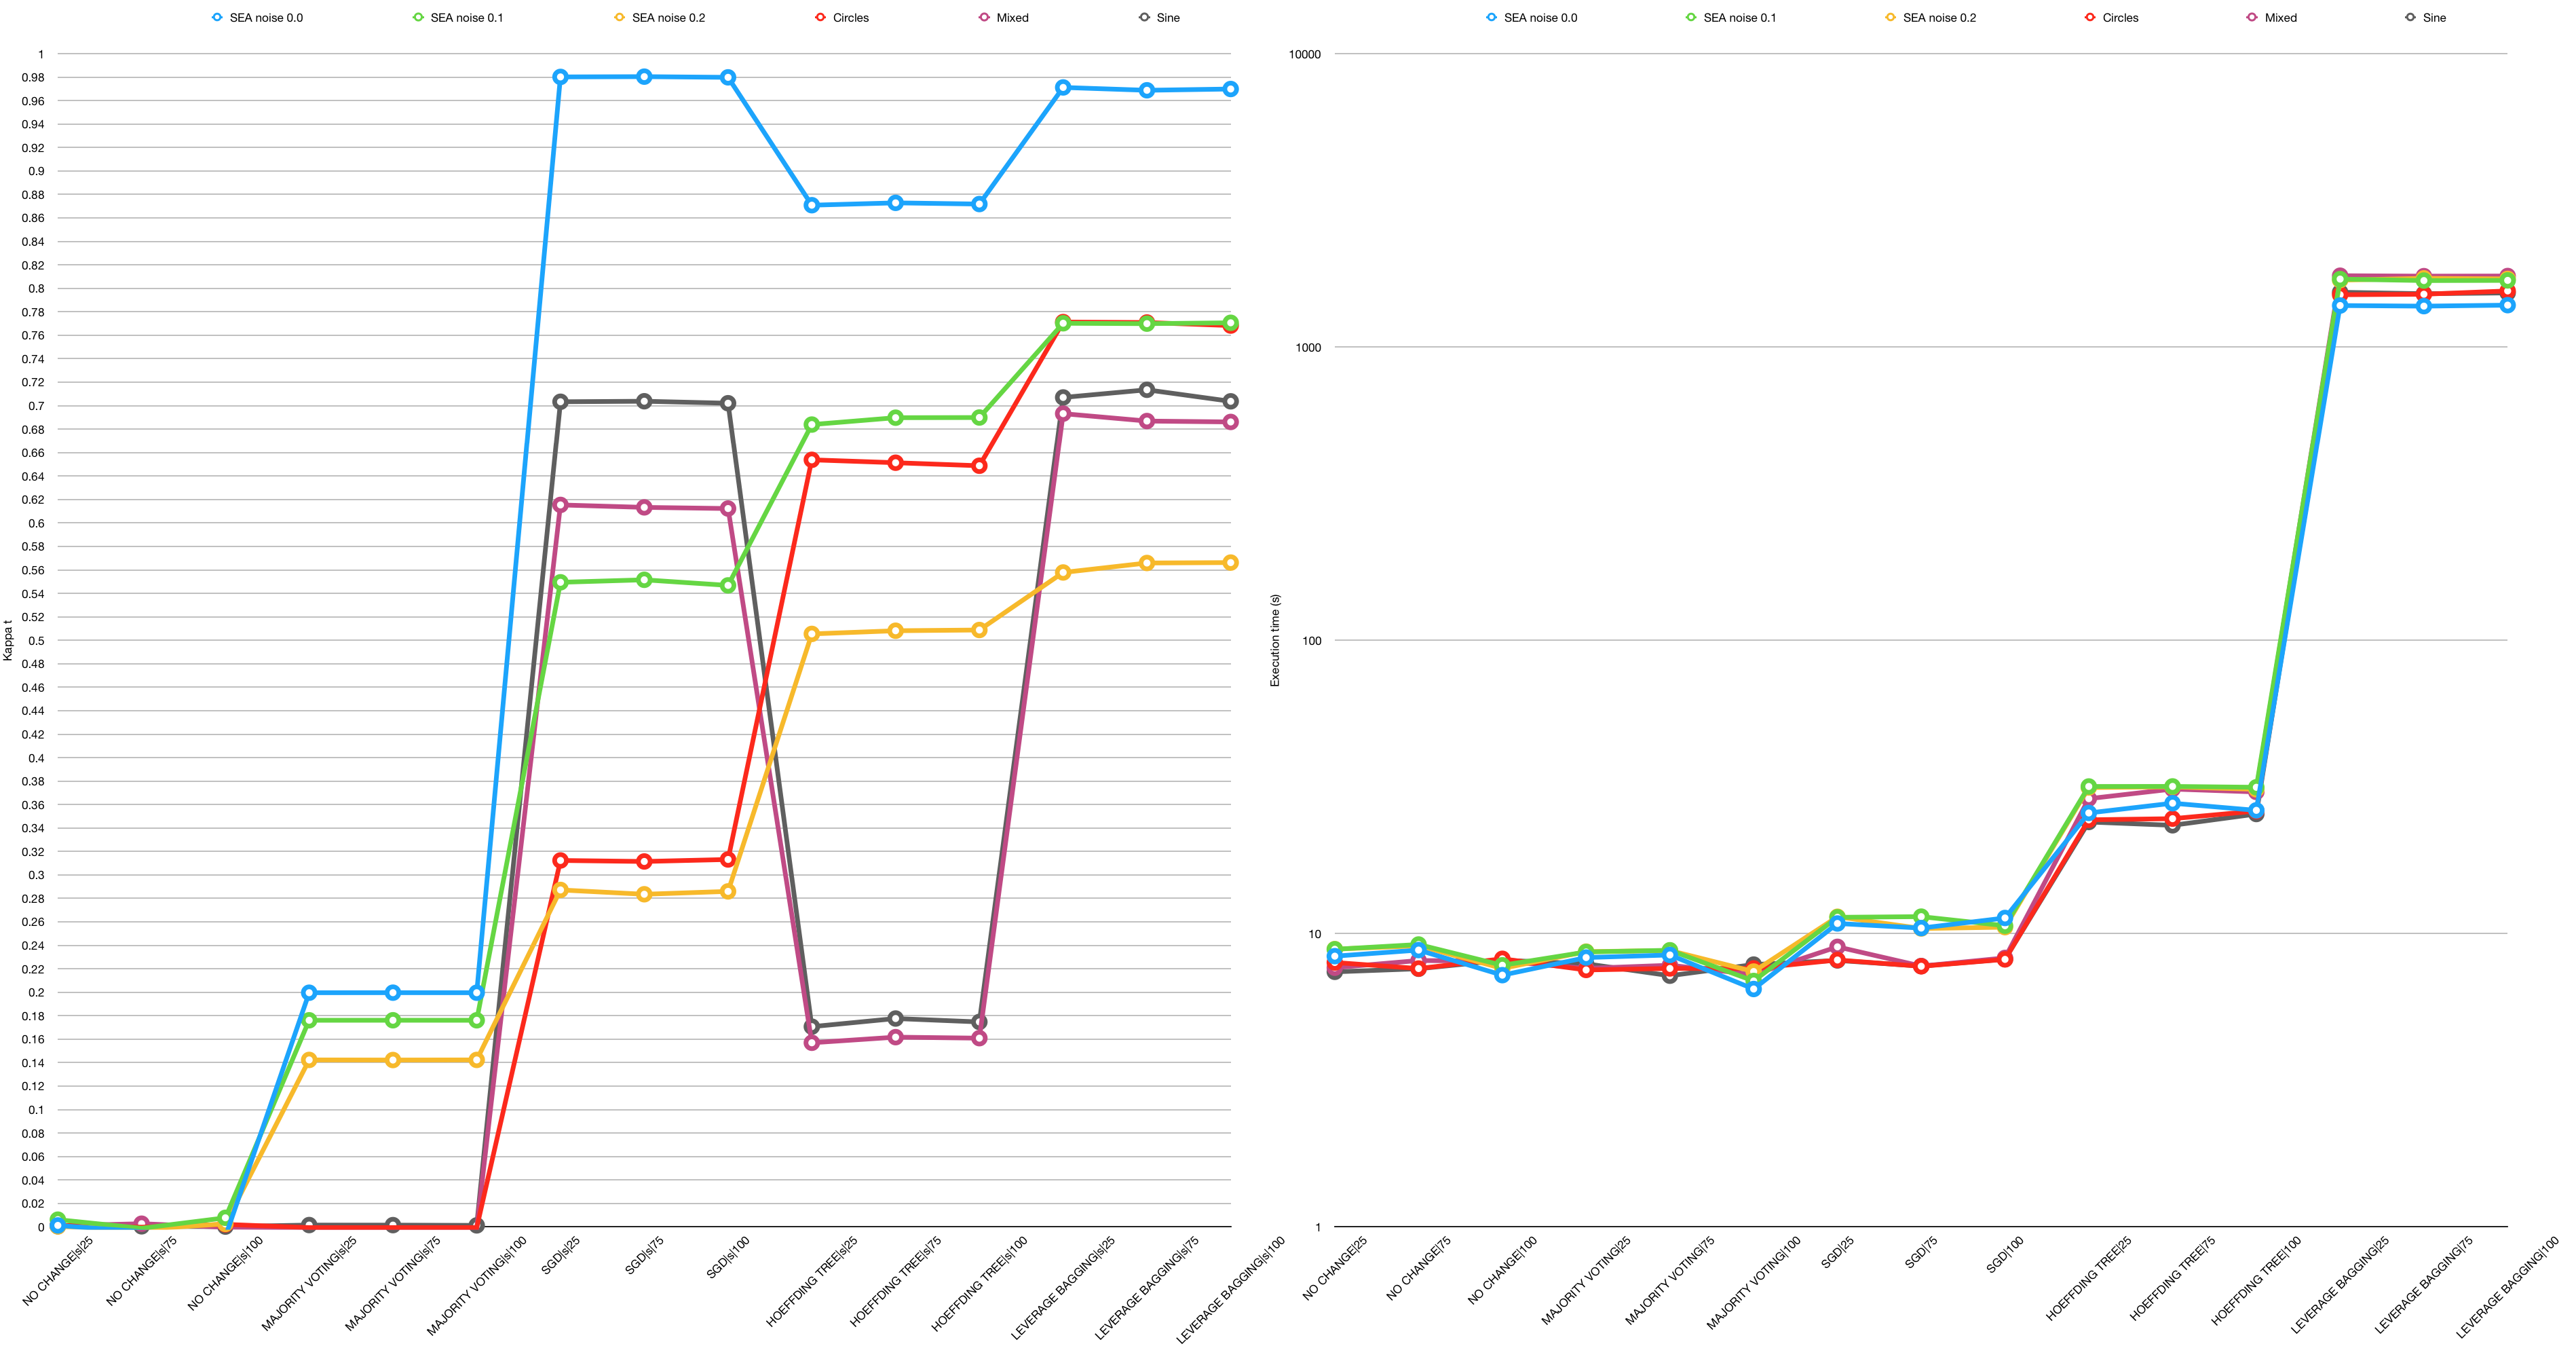
\includegraphics[width=\linewidth]{./images/chapter5/compare_sota}
\caption{\label{fig:raw_compare_sota} Comparative $\kappa_t$ and execution times with varying window sizes}
\end{figure}

Recall that we compare our LESS-TWE framework with a Leveraging Bagging ensemble with 10 Hoeffding Trees, as well as the baseline no-change and majority classifiers. For these algorithms, we made sure to use $100\%$ ground truth for the training, sliding windowing and only modified the window size, through extensive experimentation. The resulting chosen window sizes are as follows: no change (25),  majority voting (25), SGD (75), Hoeffding Tree (25), Leveraging Bagging (25). We  compare these algorithms to our voting ensemble with six different parameter combinations (1 for each increment of ground truth used, and an additional one using $100\%$ ground truth).

%However, changing the window size did not change the execution times or $\kappa_t$ by much as seen in figure \ref{fig:raw_compare_sota}. For this reason, we chose to keep one example for each algorithm, that ranked better with a given window size than the others. For the no change, majority voting, and SGD classifiers, no statistical significant difference in performance was found when changing the window size. For Hoeffding Trees, a window size of 25 showed a significant statistical difference to 100 but only for the execution time. For Leveraging Bagging, a window size of 25 showed a significant statistical difference to 100 but only for the $\kappa_t$ metric.



%\subsubsection{Visual comparison}

%Finally, we can compare our voting ensemble to the state of the art. Figure \ref{fig:raw_compare_sota_all} shows the raw results, to better visualise how each algorithm, and its parameter combinations affect the data sets that they are trying to model.

\begin{figure}
  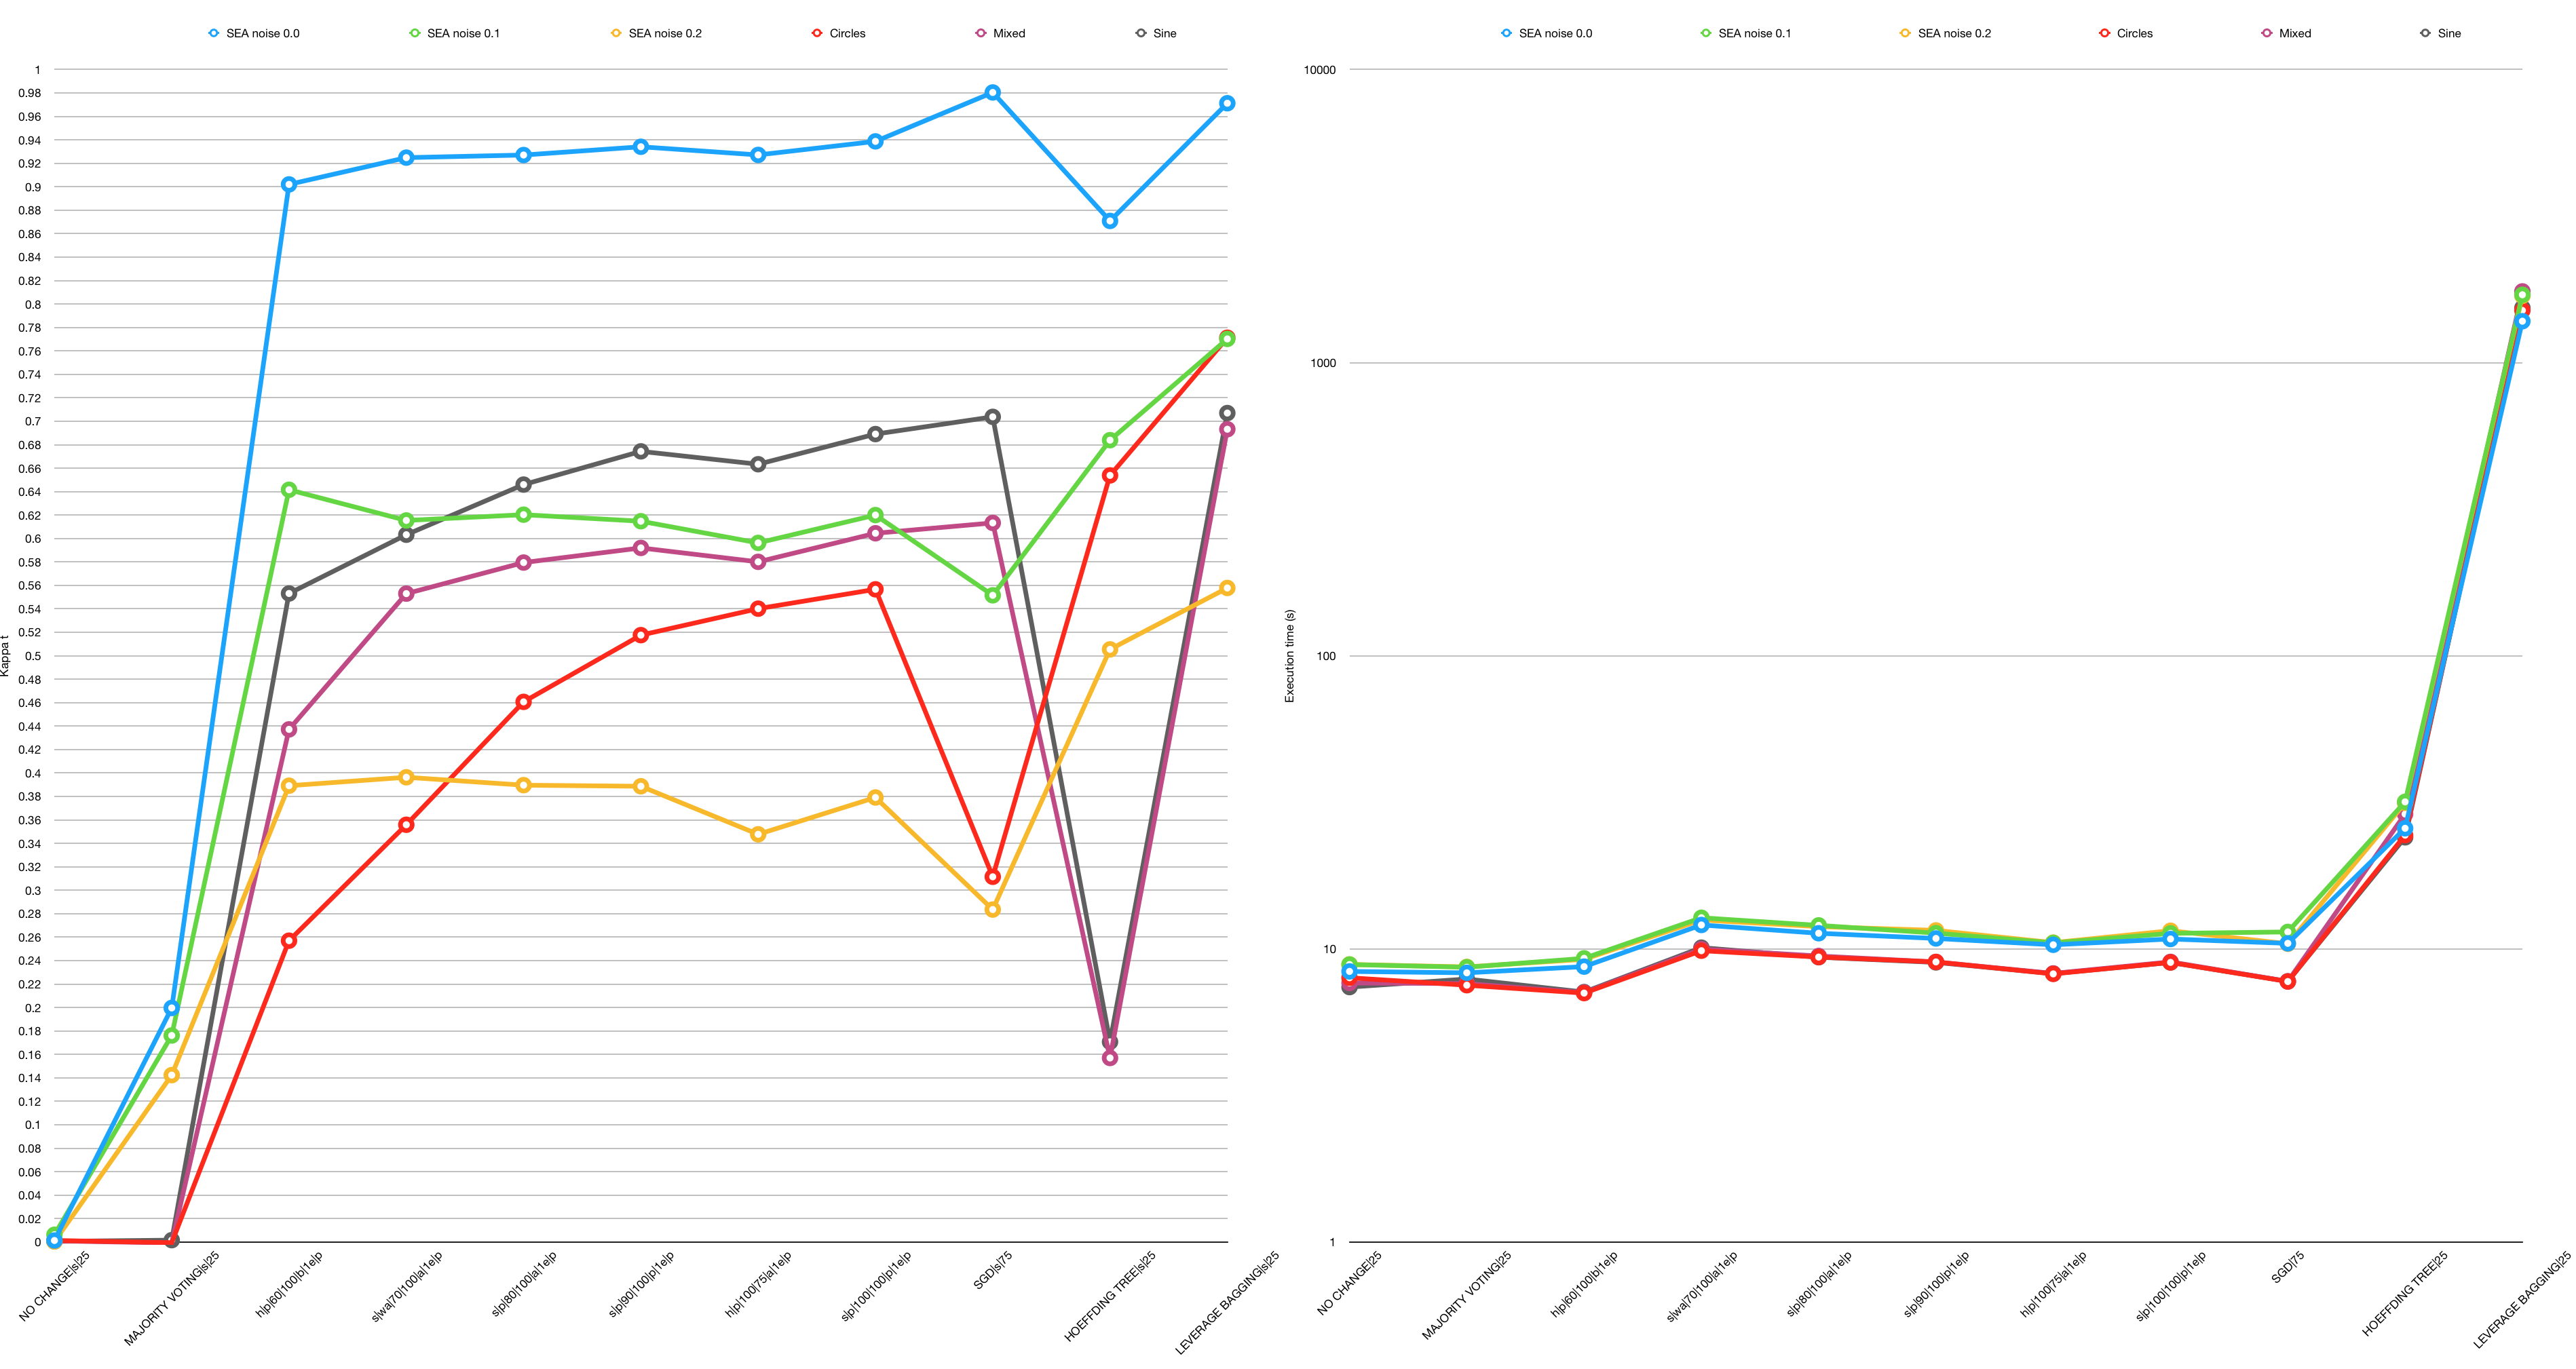
\includegraphics[width=\linewidth]{./images/chapter5/compare_sota_all}
\caption{\label{fig:raw_compare_sota_all} Comparative $\kappa_t$ and execution times}
\end{figure}

 Figures \ref{fig:raw_compare_sota} and \ref{fig:raw_compare_sota_all} shows that Leveraging Bagging (LB) does achieve the best predictive accuracy but the worst execution time. While the difference in predictive accuracy between LB and the other algorithms is noticeable, it is not glaring. However, when it comes to execution time, we were required to use a logarithmic scale to show its run time while also showing the run times of other algorithms. LB takes more than two orders of magnitude longer than the Voting Ensemble, and 1.5 orders of magnitude longer than a Hoeffding Tree (HT). Given that LB is comprised of 10 HTs, it makes perfect sense that LB takes so much longer to run.

In addition, the Friedman test, with a significance level of 0.05, yielded a value of $p < 2.1\times10^{-23}$, thus rejecting the null hypothesis that the algorithms are equivalent in terms of predictions and run times.

%However, our findings from the graph do not have the weight of a proper statistical analysis, which follows immediately.

%\subsubsection{Statistical Analysis}

%In this final section, we will test the following two null hypotheses:
%\begin{enumerate}
%\item all algorithms, with their respective parameters predict classes equally well ($\kappa_t$)
%\item all algorithms, with their respective parameters run in an equal %amount of time.
%\end{enumerate}

%\paragraph{For $\kappa_t$}

%,  the Friedman test was used, with a significance level of 0.05. We found that $p < 2.1\times10^{-23}$, thus rejecting the null hypothesis.
To determine which pairs of algorithms actually differ, we used the post-hoc Nemenyi test as shown in figure \ref{fig:sota_compare_all_kappa_nemenyi}, where a lower rank means a better predictive accuracy (a better $\kappa_t$).
The graph shows that there is no significant statistical difference between LB, our Voting Ensemble using our best overall parameter combination, an SGD classifier, and our Voting Ensemble using our hybrid windowing approach. This supports the rejection of the null hypothesis for $\kappa_t$. It is also a very good sign, because all of the above-mentioned algorithms ranked better than a single Hoeffding Tree.
Note that there is a significant statistical difference between both the majority voting and no change classifiers with all algorithms, aside from our Voting Ensemble training with $70\%$ of ground truth or less.
Therefore, this test showed that our Voting Ensemble, using our preferred parameter combinations, performed comparably, statistically speaking, to Leveraging Bagging.

\begin{figure}
  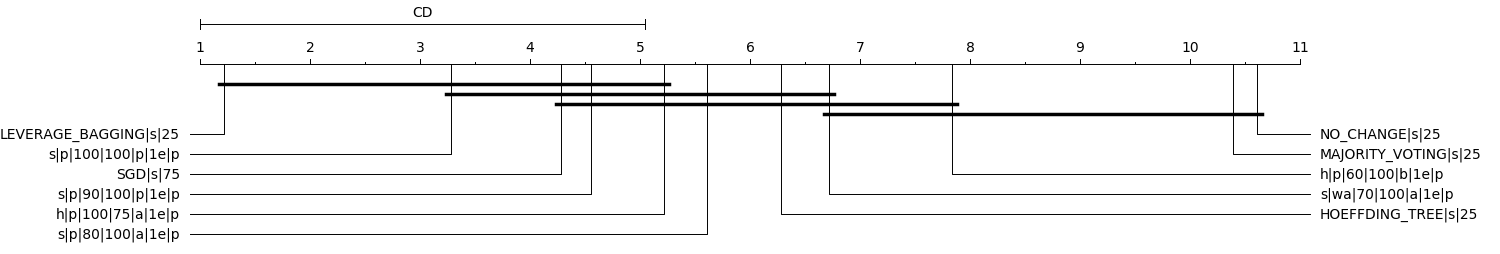
\includegraphics[width=\linewidth]{./images/chapter5/sota_compare_all_kappa_nemenyi}
\caption{\label{fig:sota_compare_all_kappa_nemenyi}Nemenyi graph ranking $\kappa_t$ for various algorithms}
\end{figure}

% A Nemenyi graph shows a ranking of algorithms on a scale from 1 to N (typically the number of algorithms compared). A bar labelled critical difference (CD) is shown above the scale, which is the minimum rank length for two algorithms to not show a significant statistical difference in rank. 
% Additionally, there may be horizontal bars that link ranked algorithms. Any algorithms that share the same horizontal bar are not significantly statistically different. Pairs of algorithms that are further apart than the CD bar are significantly statistically different.



\paragraph{Considering execution time}, we use the Friedman test again, with a significance level of 0.05. We found that $p < 1.68\times10^{-31}$, thus leaving no doubt as to the rejection of the null hypothesis. The post-hoc Nemenyi test is used to determine which pairs of algorithms differ as shown in figure  \ref{fig:sota_compare_all_execution_time_nemenyi}. The graph indicates that Leveraging Bagging ranks last, and the Hoeffding Tree ranks second last, which is as expected given the  values from figure \ref{fig:raw_compare_sota_all}.
The graph also shows that there is a significant statistical difference between Leveraging Bagging, and our Voting Ensemble. Given that Leveraging Bagging runs in over two orders of magnitude longer than our Voting Ensemble, this result is as expected. 

\begin{figure}
  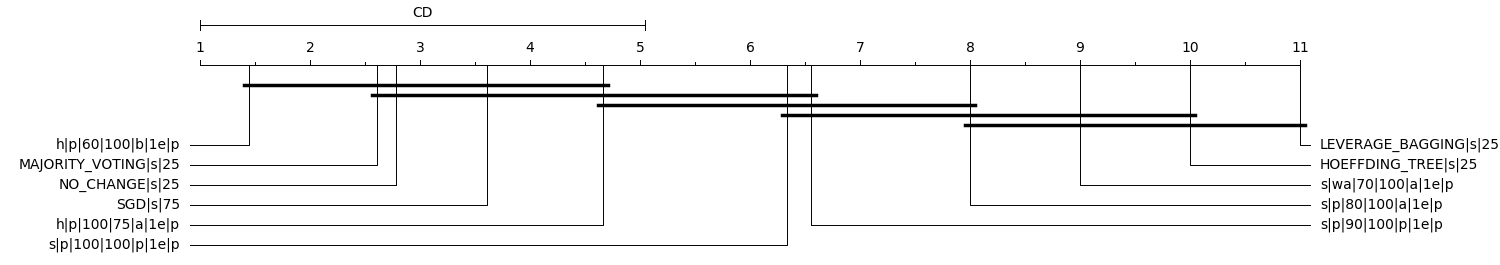
\includegraphics[width=\linewidth]{./images/chapter5/sota_compare_all_execution_time_nemenyi}
\caption{\label{fig:sota_compare_all_execution_time_nemenyi}Nemenyi graph ranking execution times for various algorithms}
\end{figure}



%\subsubsection{Discussion}
In summary, 
statistical significance tests show that our Voting Ensemble is able to outperform the Leveraging Bagging algorithm in execution time, and that it is able to perform on par with \textit{Leveraging Bagging} in regards to the $\kappa_t$ measured metric. It also indicated that the predictive performance of our ensemble when trained with only $90\%$ ground truth does not present a statistical significant difference to that of \textit{Leveraging Bagging}. Our results further show that the predictive accuracy of our ensemble when training on data sets containing less than 80\% labelled data approaches the traditional threshold for statistical significance, and presents no significant difference when using a significance value of $0.01$.
Our results indicate that our algorithm  predicts comparably to Leveraging Bagging and brings outstanding time savings in algorithm execution-time, running approximately 160 times faster. Practically, this means that our ensemble should definitely be considered when execution time is an important metric, since the predictive performance is comparable to that of Leveraging Bagging.




\section{Conclusion\label{section:conclusion}}
This paper focused on improving semi-supervised learning from evolving streams without the use of clustering techniques, which are computationally expensive \cite{krempl2014open}. The goal of this study was to design fast algorithms to work with fewer labelled examples, and to extend an existing algorithm to detect drifts without relying on ground truth. Experiments were conducted in order to compare the performance of our framework against that of the state of the art in terms of predictive accuracy and execution time, while considering the percentage of labelled instances used at each stage of learning. 

Future work will include introducing an active-learning approach to determine if further reductions in labelled data can be achieved, and by how much; addressing the memory issues of weighted summarising classifiers to better "forget" and relearn old knowledge; and resolve the lack of ensemble classifier diversity guarantees by substituting cyclical for stochastic training from novel windows.

\printbibliography

\end{document}
